% ============================================== %

%%%%%%%%%%%%%%%%%%%%%%%%%%%%%%%%%%%%%%%%%%%%%%%%%%
%%%			  04 Trabalho Prático 04		   %%%
%%%%%%%%%%%%%%%%%%%%%%%%%%%%%%%%%%%%%%%%%%%%%%%%%%

% ============================================== %

\section{Trabalho Prático 04}


Para a viga engastada com momento constante aplicado na extremidade livre pede-se:

\begin{itemize}
	\item[a)] Traçar os gráficos $M\times \theta$, $M\times u$, $M\times v$ para
	$\pi \in \left[0, 2\pi\right]$ rad no ponto $x=L$
	\item[b)] Detalhar a solução da viga deformada para $\theta = \pi$ e
	$\theta = 2\pi$, considerando-se 11 pontos igualmente espaçados (10 elementos)
	ao longo do comprimento da viga.
\end{itemize}

Adotar:
$$
\left\{\begin{array}{lcl}
	EI &=& 4\times 10^4\text{ N/cm} \\
	L &=& 500\text{ cm} \\
	\Delta\theta &=& \frac{\pi}{36}\:\:\text{rad} \\
\end{array}\right.
$$

\begin{figure}[H]
	\centering
	\caption{Sistema estrutural do Trabalho Prático 04.}
	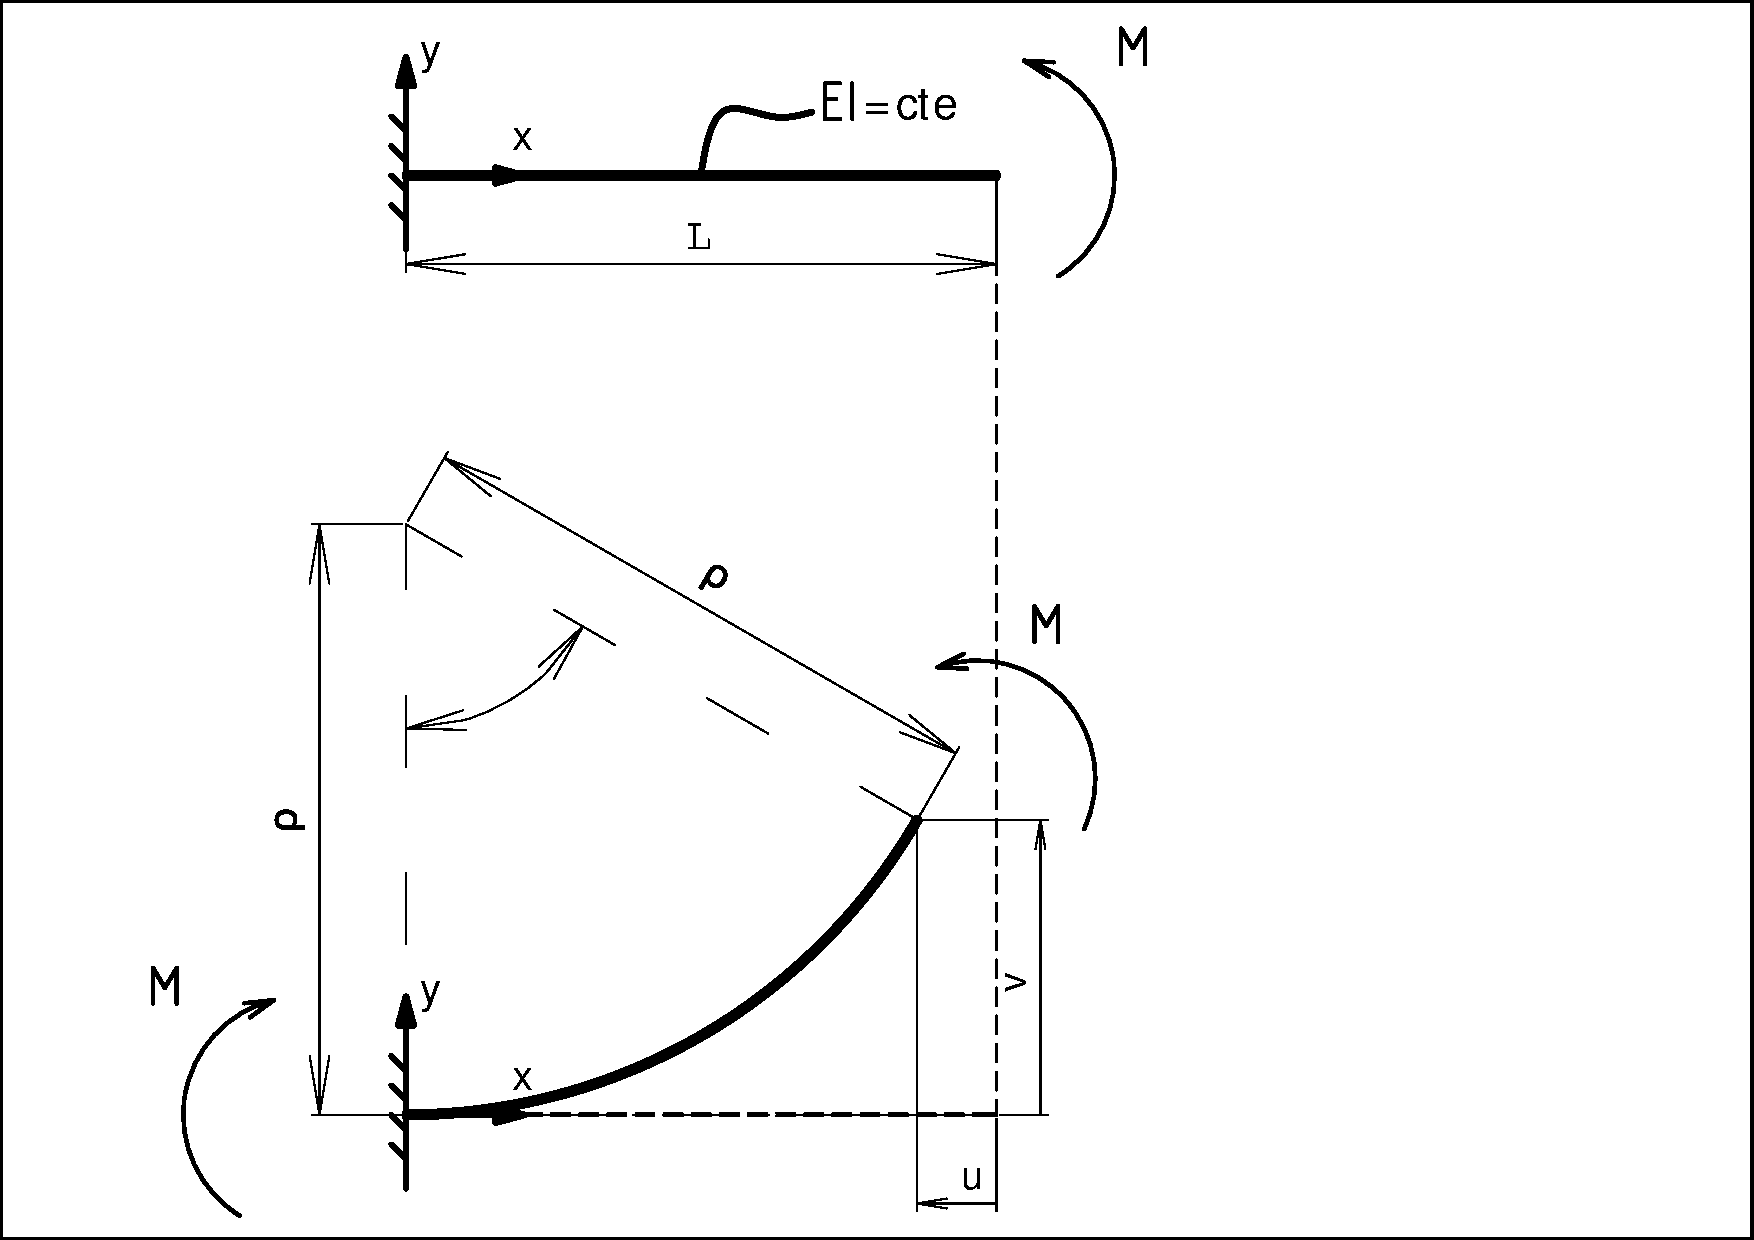
\includegraphics[
		trim=25mm 3mm 100mm 4mm,
		clip,
		width=0.75\textwidth
	]{figuras/TPs-4.pdf}
\end{figure}


% ================ Resolução TP-04 ================
\begin{textocaixa}
\hspace{10mm}




\end{textocaixa}